%% AI6103 Homework Assignment report (AAAI two-column format).
%% Requires the official AAAI-24 author kit files in this folder: aaai24.sty and aaai24.bst
%% (https://aaai.org/authorkit24-2/). Discussion text is left as \todo{} markers.
\documentclass[letterpaper]{article}
\usepackage{aaai24}
\ifdefined\XeTeXversion
% XeTeX (tectonic) preview only: Times-metric clones of what pdfLaTeX gets from times/helvet/courier
\usepackage{fontspec}
\setmainfont{texgyretermes-regular.otf}[BoldFont=texgyretermes-bold.otf,ItalicFont=texgyretermes-italic.otf,BoldItalicFont=texgyretermes-bolditalic.otf]
\setsansfont{texgyreheros-regular.otf}[BoldFont=texgyreheros-bold.otf,ItalicFont=texgyreheros-italic.otf,BoldItalicFont=texgyreheros-bolditalic.otf]
\setmonofont{texgyrecursor-regular.otf}[BoldFont=texgyrecursor-bold.otf,ItalicFont=texgyrecursor-italic.otf,BoldItalicFont=texgyrecursor-bolditalic.otf]
\else
\usepackage{times}
\usepackage{helvet}
\usepackage{courier}
\fi
\usepackage[hyphens]{url}
\usepackage{graphicx}
\urlstyle{rm}
\def\UrlFont{\rm}
\usepackage{natbib}
\usepackage{caption}
\frenchspacing
\ifdefined\pdfpagewidth
\setlength{\pdfpagewidth}{8.5in}
\setlength{\pdfpageheight}{11in}
\fi
\usepackage{amsmath}
\usepackage{booktabs}
\usepackage{placeins}
\usepackage{xcolor}
\usepackage{pgfplots}
\pgfplotsset{compat=1.16}
\usepackage{listings}
\lstset{basicstyle={\scriptsize\ttfamily},numbers=left,numberstyle=\tiny,numbersep=4pt,
  aboveskip=0pt,belowskip=0pt,showstringspaces=false,tabsize=2,breaklines=true,
  breakatwhitespace=true,columns=fullflexible,keepspaces=true,frame=single,framesep=1pt}
\ifdefined\pdfinfo
\pdfinfo{/TemplateVersion (2024.1)}
\fi
\setcounter{secnumdepth}{2}

% Placeholder for text to be written by hand.
\newcommand{\todo}[1]{\textcolor{red}{\textit{[#1]}}}

\title{AI6103 Homework: Effects of Learning Rate, Schedule, Weight Decay and Mixup\\on EfficientNetV2-S for Dog Breed Identification}
\author{Ayush Bhatt\\Matric.\ No.\ G2610412E\\ Nanyang Technological University}
\begin{document}
\maketitle

\section{Introduction}
We train EfficientNetV2-S \cite{tan2021} from scratch on the Dog Breed Identification dataset \cite{dogbreed} (120 breeds; 7,155/1,533/1,534 train/val/test images) using SGD with momentum 0.9, implemented in PyTorch \cite{paszke2019}. All hyperparameters are tuned on the validation set; the test set is used once at the end. All runs use batch size 128, seed 0, and the cross-entropy loss with label smoothing 0.1. Metrics are logged per epoch (training metrics are running averages over the augmented mini-batches of that epoch). Generative AI (Claude Sonnet 5.5 \cite{claude2026}) was used to help prepare the LaTeX report, format tables and figures, and give feedback on draft text; all experiments, analysis and final wording are my own.


\section{Data Preprocessing}
Images are resized to $100\times100$. Channel statistics are computed on the training set (pixel values in $[0,1]$) and used to normalise all splits (Table~\ref{tab:norm}). Training images are augmented with a random horizontal flip ($p=0.5$) and a random $100\times100$ crop of the image zero-padded by 12 pixels on all sides. The code is shown in Listing~\ref{lst:code}.

\begin{table}[ht]
\centering
\footnotesize\setlength{\tabcolsep}{3pt}
\begin{tabular}{lccc}
\toprule
 & R & G & B\\
\midrule
Mean & 0.4772 & 0.4528 & 0.3928\\
Std & 0.2534 & 0.2480 & 0.2523\\
\bottomrule
\end{tabular}
\caption{Per-channel mean and standard deviation of the training set.}
\label{tab:norm}
\end{table}

\begin{lstlisting}[language=Python,caption={Data preprocessing and augmentation.},label={lst:code},captionpos=b]
resize = v2.Resize((100, 100), antialias=True)
imgs = torch.stack([resize(decode_image(
    f'./data/train/images/{p}.jpg',
    mode=ImageReadMode.RGB))
    for p in trainDf.id]).to(device)  # uint8
x = imgs.float() / 255
mean = x.mean(dim=(0, 2, 3))
std = x.std(dim=(0, 2, 3))
norm = v2.Normalize(mean.tolist(), std.tolist())
PAD = 12

def augment(xb):  # xb: uint8 (B,C,H,W) on GPU
  B, _, H, W = xb.shape
  dev = xb.device
  flip = torch.rand(B, device=dev) < 0.5
  xb = torch.where(flip[:, None, None, None],
                   xb.flip(3), xb)  # h-flip, p=0.5
  xp = F.pad(xb, (PAD, PAD, PAD, PAD))  # zero pad
  dy = torch.randint(0, 2*PAD+1, (B,), device=dev)
  dx = torch.randint(0, 2*PAD+1, (B,), device=dev)
  rows = dy[:, None] + torch.arange(H, device=dev)
  cols = dx[:, None] + torch.arange(W, device=dev)
  b = torch.arange(B, device=dev)[:, None, None]
  out = xp[b, :, rows[:, :, None], cols[:, None, :]]
  return out.permute(0, 3, 1, 2)  # (B,C,H,W)

def prep(xb, train=False):
  if train: xb = augment(xb)
  return norm(xb.float() / 255)
\end{lstlisting}

\section{Learning Rate}
Three runs with initial learning rate $0.5$, $0.05$ and $0.001$; no weight decay, no schedule, 15 epochs. Final-epoch results are in Table~\ref{tab:lr} and the curves in Figure~\ref{fig:lr}.

\begin{table}[ht]
\centering
\footnotesize\setlength{\tabcolsep}{3pt}
\begin{tabular}{lcccc}
\toprule
LR & Train loss & Train acc & Val loss & Val acc\\
\midrule
0.5   & 4.5881 & 7.98\% & 4.8432 & 5.41\%\\
0.05  & 4.9521 & 3.42\% & 4.9880 & 3.52\%\\
0.001 & 6.8610 & 0.73\% & 6.8901 & 0.52\%\\
\bottomrule
\end{tabular}
\caption{Final (epoch 15) losses and accuracies for different initial learning rates.}
\label{tab:lr}
\end{table}

\begin{figure*}[!tb]
\centering
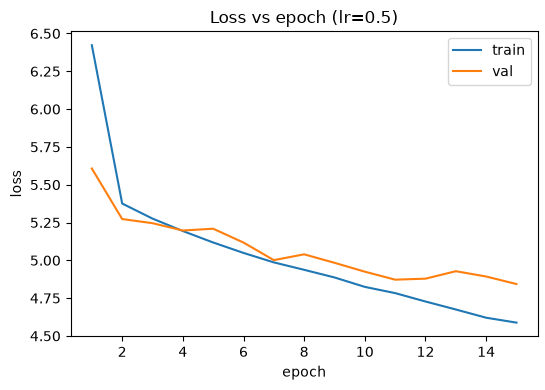
\includegraphics[width=0.325\textwidth]{figures/crops/lr0.5_loss.png}\hfill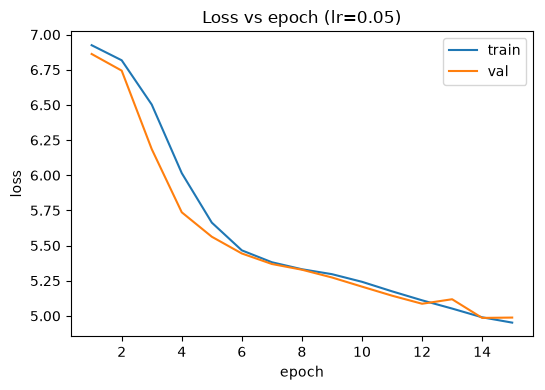
\includegraphics[width=0.325\textwidth]{figures/crops/lr0.05_loss.png}\hfill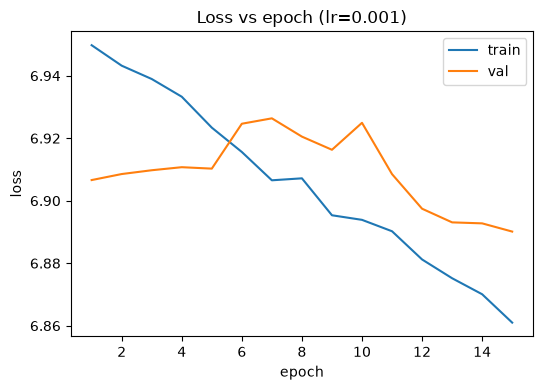
\includegraphics[width=0.325\textwidth]{figures/crops/lr0.001_loss.png}\\[2pt]
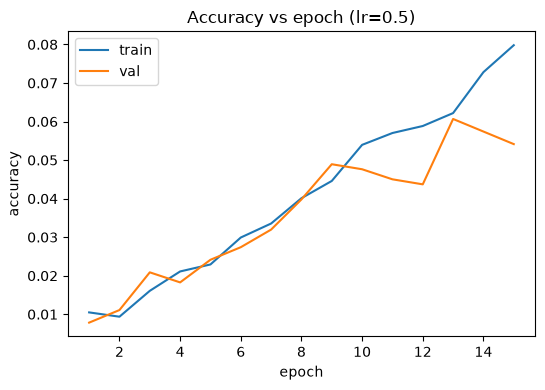
\includegraphics[width=0.325\textwidth]{figures/crops/lr0.5_acc.png}\hfill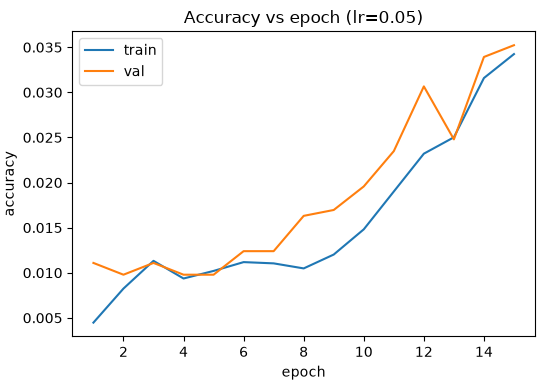
\includegraphics[width=0.325\textwidth]{figures/crops/lr0.05_acc.png}\hfill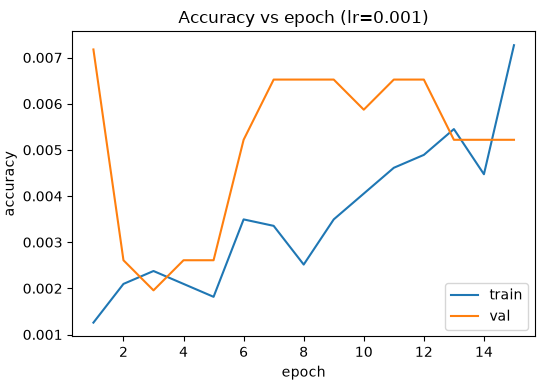
\includegraphics[width=0.325\textwidth]{figures/crops/lr0.001_acc.png}
\caption{Training/validation loss (top) and accuracy (bottom) vs.\ epoch for initial learning rate 0.5, 0.05 and 0.001 (left to right), 15 epochs.}
\label{fig:lr}
\end{figure*}

% \todo{Which learning rate is best for training loss/accuracy and for validation loss/accuracy, and why.}\\
The best learning rate for both validation and training, loss and accuracy, is lr=0.5. For training, the major factor in increasing accuracy and lowering loss is the ability to fit our model quickly, and at such a low number of epochs (15) this happens best when our learning rate is 0.5 as it allows us to take the biggest steps, among the given options, towards lower loss. For validation, and during early training, the major contributor of better accuracy is being able to improve our training loss and accuracy. Also, at 15 epochs overfitting will be negligible. Hence, validation loss and accuracy will follow the trend of training loss and accuracy. For other lower learning rate options we are not able to take big enough steps in 15 epochs which contributes to training and validation loss being not as good as our best performer. Comparing our best and second best performer's accuracies, we see that $\Delta$ Training = 4.56 points and $\Delta$ Validation = 1.89 points.


\section{Learning Rate Schedule}
\subsection{Cosine Annealing}
Cosine annealing \cite{loshchilov2017} is a learning rate schedule. With initial learning rate $\eta_0$ and $T$ total optimisation steps, the learning rate at step $t$ is
\begin{equation}
\eta_t=\tfrac{1}{2}\eta_0\left(1+\cos\frac{\pi t}{T}\right),
\label{eq:cos}
\end{equation}
so $\eta_0$ decays smoothly to $0$ at $t=T$ (Figure~\ref{fig:sched}). Here $T=300\times\lceil 7155/128\rceil=16{,}800$ and the scheduler is stepped after every mini-batch.
% \todo{Intuitive description of cosine annealing.}
It builds on the step-down schedule, removing the abruptness of step-down and making it smoother. As observed from Eq.~\ref{eq:cos}, it decreases learning rate slowly at first, then fastest in the middle and lastly it slows down in lowering the learning rate. This helps because it makes the steps at start take bigger steps for faster drop and again slows the decreasing at end which helps in converging the weights near minimum.

\begin{figure}[ht]
\centering
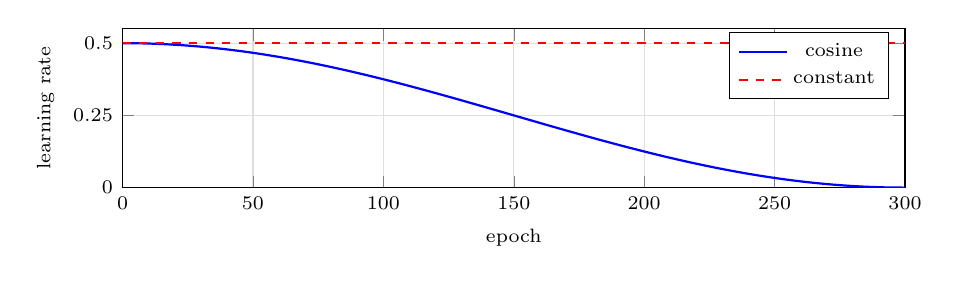
\begin{tikzpicture}
\begin{axis}[width=0.95\columnwidth,height=3.6cm,xlabel={epoch},ylabel={learning rate},
  xmin=0,xmax=300,ymin=0,ymax=0.55,tick label style={font=\scriptsize},label style={font=\scriptsize},
  ytick={0,0.25,0.5},grid=both,grid style={gray!25}]
\addplot[blue,thick,domain=0:300,samples=100] {0.25*(1+cos(180*x/300))};
\addplot[red,dashed,thick,domain=0:300] {0.5};
\legend{\scriptsize cosine,\scriptsize constant}
\end{axis}
\end{tikzpicture}
\caption{Learning rate schedules used in Section~4 ($\eta_0=0.5$).}
\label{fig:sched}
\end{figure}

\subsection{Experiments}
Using the best learning rate $\eta_0=0.5$ (best in Section 3), we train for 300 epochs with (1) a constant learning rate and (2) cosine annealing to zero. Results are in Table~\ref{tab:sched} and Figure~\ref{fig:sched2}.

\begin{table}[ht]
\centering
\footnotesize\setlength{\tabcolsep}{3pt}
\begin{tabular}{lcccc}
\toprule
Setting & Train loss & Train acc & Val loss & Val acc\\
\midrule
Constant LR & 1.0381 & 99.93\% & 5.5300 & 19.77\%\\
Cosine      & 1.0469 & 99.93\% & 5.4822 & 20.74\%\\
\bottomrule
\end{tabular}
\caption{Final (epoch 300) results with constant learning rate vs.\ cosine annealing ($\eta_0=0.5$).}
\label{tab:sched}
\end{table}

\begin{figure*}[!tb]
\centering
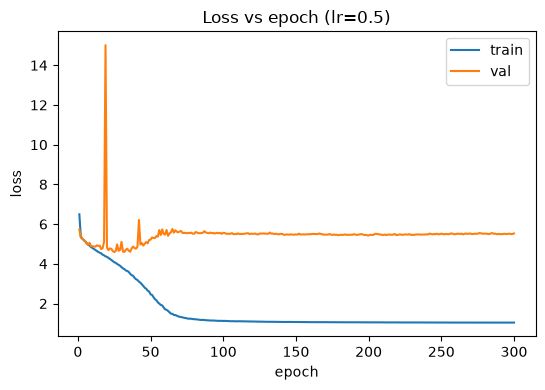
\includegraphics[width=0.42\textwidth]{figures/crops/nocosine_loss.png}\hfill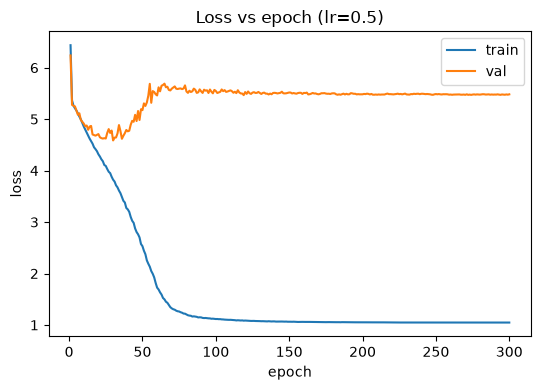
\includegraphics[width=0.42\textwidth]{figures/crops/cosine_loss.png}\\[2pt]
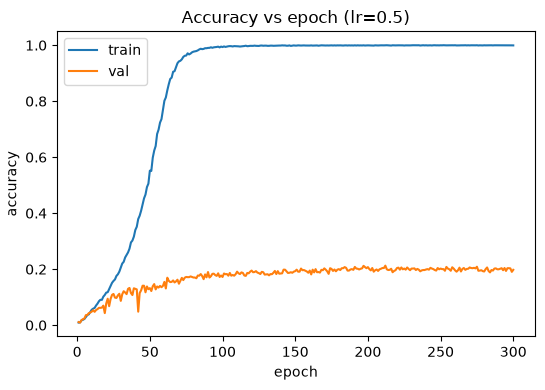
\includegraphics[width=0.42\textwidth]{figures/crops/nocosine_acc.png}\hfill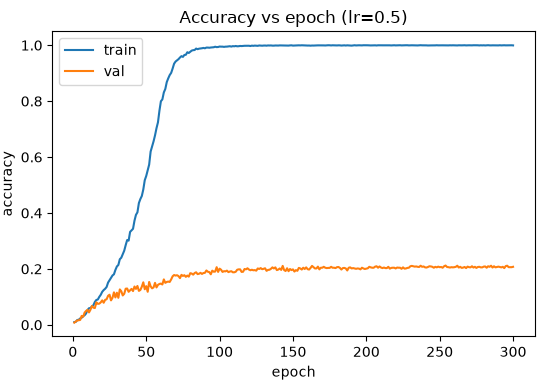
\includegraphics[width=0.42\textwidth]{figures/crops/cosine_acc.png}
\caption{Training/validation loss (top) and accuracy (bottom) vs.\ epoch for a constant learning rate (left) and cosine annealing (right), $\eta_0=0.5$, 300 epochs.}
\label{fig:sched2}
\end{figure*}

% \todo{Findings and discussion of the differences between the two schedules.}
According to Table~\ref{tab:sched}, training accuracy for constant learning rate vs cosine annealing is almost the same, $\Delta \approx 0$, while for validation cosine annealing is only slightly better, $\Delta = 0.97$ points. A constant learning rate of 0.5 stays large till the end, so the weights keep bouncing around and stay noisier. Cosine decays the rate to zero, so the last epochs take small steps and the weights settle into a minimum. That settled solution may generalise a bit better, giving slightly lower validation loss and higher accuracy, but the difference is below one point of accuracy, which is small compared to run-to-run variation, so this is only weak evidence. It is a convergence effect, not a regularisation effect. Cosine does not stop overfitting, since both runs still overfit. From Figure~\ref{fig:sched2}, we can infer that while training shows similar trends for both (numbers differ just trends are compared), validation shows difference in that for constant we converge much more noisily than we do after applying scheduler.


\section{Weight Decay}
Cosine annealing with $\eta_0=0.5$ and weight decay $\lambda\in\{5\times10^{-4},\,1\times10^{-4}\}$, 300 epochs. Results are in Table~\ref{tab:wd} and Figure~\ref{fig:wd}.

\begin{table}[ht]
\centering
\footnotesize\setlength{\tabcolsep}{3pt}
\begin{tabular}{lcccc}
\toprule
$\lambda$ & Train loss & Train acc & Val loss & Val acc\\
\midrule
$5\times10^{-4}$ & 1.0627 & 99.99\% & 3.9221 & 34.96\%\\
$1\times10^{-4}$ & 1.0416 & 99.94\% & 4.9891 & 24.98\%\\
\bottomrule
\end{tabular}
\caption{Final (epoch 300) results for two weight decay coefficients.}
\label{tab:wd}
\end{table}

\begin{equation}
  W = W - \eta \lambda W
  \label{wd}
\end{equation}

\begin{figure*}[!tb]
\centering
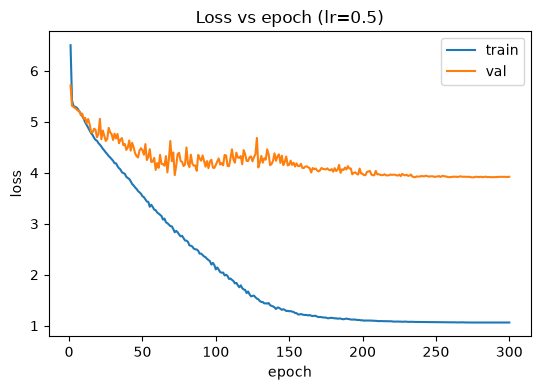
\includegraphics[width=0.42\textwidth]{figures/crops/wd5e4_loss.png}\hfill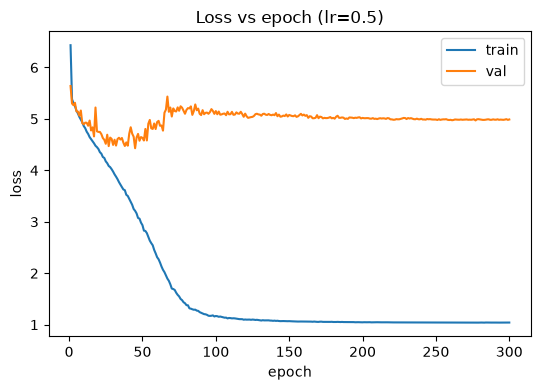
\includegraphics[width=0.42\textwidth]{figures/crops/wd1e4_loss.png}\\[2pt]
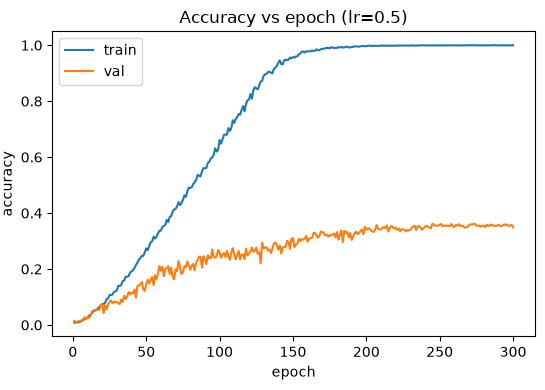
\includegraphics[width=0.42\textwidth]{figures/crops/wd5e4_acc.png}\hfill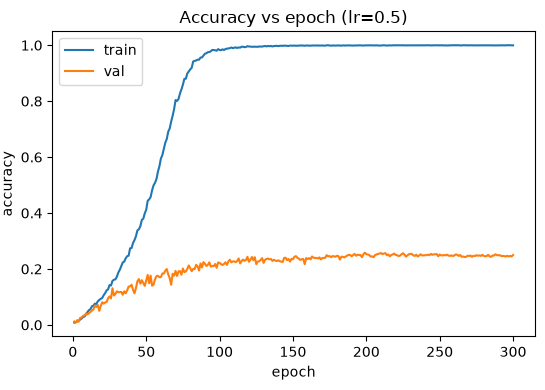
\includegraphics[width=0.42\textwidth]{figures/crops/wd1e4_acc.png}
\caption{Training/validation loss (top) and accuracy (bottom) vs.\ epoch for weight decay $\lambda=5\times10^{-4}$ (left) and $1\times10^{-4}$ (right), with cosine annealing, 300 epochs.}
\label{fig:wd}
\end{figure*}

% \todo{Findings and discussion of the regularisation effect of weight decay.}
From all our recent findings we can see that our model overfits our training data and the gap between training and validation accuracy is huge $\Delta$ = 79 points. So we introduce a regularisation technique called weight decay, which penalizes larger values of weights (Eq.~\eqref{wd}). This encourages them to be smaller and in turn it helps in generalizing since larger weights tend to help reach the values which might be exceptions, this does not solve overfitting completely just helps in reducing it ($\Delta$ train-val = 65 points). Thus, after applying weight decay we can see a good amount of improvement $\Delta$ = $+14.22$ points, which is a $68.6$\% relative improvement. The larger weight decay here helps in better penalization of larger weights thus being better in validation accuracy which can be observed in Table~\ref{tab:wd}. This suggests that our weights were adapting to the exceptions/outliers in our data and hence overfitting. So, even a smaller $\lambda=1\times10^{-4}$ gives a clear gain (+20.4\% relative), but the larger value gives a better gain ($+68.6$\% relative). Figure~\ref{fig:wd} shows that both $\lambda$ show similar trends in training but vary considerably in validation. For $\lambda=1\times10^{-4}$ the training loss barely changes from cosine annealing, 1.0469 without weight decay vs 1.0416 with it, but the validation loss improves from 5.4822 to 4.9891. With $\lambda=5\times10^{-4}$ training loss slightly worsens and validation loss greatly improves at train\_loss = 1.0627 and val\_loss = 3.9221.

\section{Data Augmentation: Mixup}
Mixup \cite{zhang2018} trains on convex combinations of random example pairs,
\begin{equation}
\begin{aligned}
\tilde{x}&=\lambda x_i+(1-\lambda)x_j,\\
\tilde{y}&=\lambda y_i+(1-\lambda)y_j,\quad
\lambda\sim\mathrm{Beta}(\alpha,\alpha),
\end{aligned}
\end{equation}
with $\alpha=0.2$. The density of $\mathrm{Beta}(0.2,0.2)$ is shown in Figure~\ref{fig:beta}. We apply mixup on top of flip and crop augmentation, with the best setup so far (cosine annealing, $\eta_0=0.5$, $\lambda_{\mathrm{wd}}=5\times10^{-4}$, 300 epochs). Training accuracy is computed against the dominant class of the mixed label; validation uses the clean images. Results are in Table~\ref{tab:mixup} and Figure~\ref{fig:mixup}.

\begin{figure}[ht]
\centering
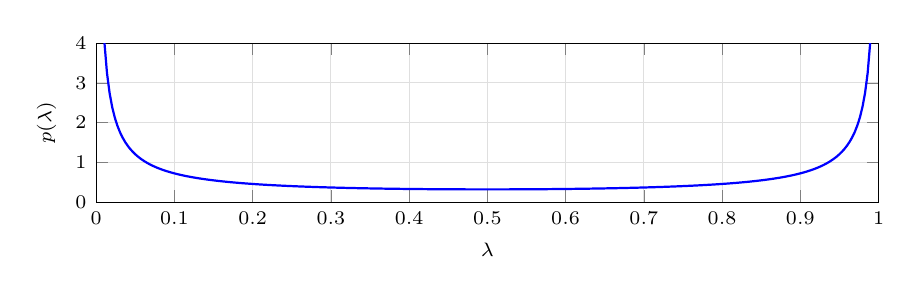
\begin{tikzpicture}
\begin{axis}[width=0.95\columnwidth,height=3.6cm,xlabel={$\lambda$},ylabel={$p(\lambda)$},
  xmin=0,xmax=1,ymin=0,ymax=4,tick label style={font=\scriptsize},label style={font=\scriptsize},
  grid=both,grid style={gray!25}]
\addplot[blue,thick,domain=0.004:0.996,samples=300] {0.10526*x^(-0.8)*(1-x)^(-0.8)};
\end{axis}
\end{tikzpicture}
\caption{Probability density of $\mathrm{Beta}(\alpha{=}0.2,\beta{=}0.2)$, $p(\lambda)=\frac{\Gamma(0.4)}{\Gamma(0.2)^2}\lambda^{-0.8}(1-\lambda)^{-0.8}$.}
\label{fig:beta}
\end{figure}

\begin{table}[ht]
\centering
\footnotesize\setlength{\tabcolsep}{3pt}
\begin{tabular}{lcccc}
\toprule
Setting & Train loss & Train acc & Val loss & Val acc\\
\midrule
Mixup ($\alpha=0.2$) & 1.9781 & 90.62\% & 3.6858 & 25.77\%\\
\midrule
\multicolumn{2}{l}{Test accuracy} & \multicolumn{3}{l}{27.38\%}\\
\bottomrule
\end{tabular}
\caption{Final (epoch 300) results with mixup and accuracy on the hold-out test set.}
\label{tab:mixup}
\end{table}

\begin{figure*}[!tb]
\centering
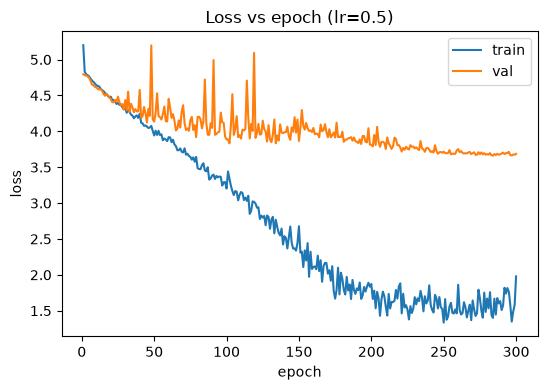
\includegraphics[width=0.42\textwidth]{figures/crops/mixup_loss.png}\hfill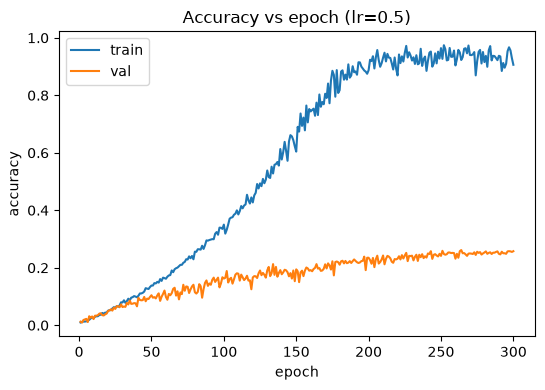
\includegraphics[width=0.42\textwidth]{figures/crops/mixup_acc.png}
\caption{Training/validation loss (left) and accuracy (right) vs.\ epoch with mixup ($\alpha=0.2$), 300 epochs.}
\label{fig:mixup}
\end{figure*}

% \todo{Findings and discussion of the effect of mixup.}
From our previous findings with weight decay we know that regularisation is the right track to improve our overfitting problem. So we introduce another regularisation technique, mixup. Mixup is a technique that mixes raw input data with different labels to create a new input to be fed to our model during training. It helps by softening the decision boundary between labels, which can help reduce overfitting. This softening of decision boundary penalizes the model when it tries tilting towards the noise and exceptions. With $\alpha=0.2$ the mixing coefficient $\lambda\sim\mathrm{Beta}(0.2,0.2)$ is usually close to 0 or 1 (Figure~\ref{fig:beta}), so most mixed samples stay close to one of the two original images, which keeps the regularisation mild. From Table~\ref{tab:mixup}, we observe that after introducing mixup our training accuracy takes a hit and decreases 9 points. This worsened training accuracy occurs because we are mixing data and creating soft new labels which then get compared against the dominant class, which is why the training accuracy drops (the final-epoch training metrics with mixup also fluctuate noticeably between epochs, so these changes are approximate). For validation, on the other hand, we do not see any improvement rather we see a decrease of accuracy from 34.96\% to 25.77\%, though validation loss decreased marginally about 6\% from 3.92 to 3.69. From our Figure~\ref{fig:mixup} we can also observe that validation loss is highly fluctuating with spikes around first 150 epochs. The gap between training and validation accuracy is essentially unchanged, 65.0 points without mixup (99.99 $-$ 34.96) and 64.9 points with it (90.62 $-$ 25.77), so mixup did not reduce our overfitting here. Overall, mixup might not be the best technique to use for our dataset. A possible reason is that with $\alpha=0.2$ most mixes are mild, and on top of weight decay and cosine annealing it adds little. The final test accuracy is 27.38\%, close to the validation accuracy of 25.77\%. This test accuracy is to be expected on new images considering similar validation accuracy.

\FloatBarrier
\bibliography{refs}

\end{document}
